The balloons will be located in the stratosphere, approximately 20 kilometers above the earth's surface \citep{}. The stratosphere is a collection of layers, each with a different jet stream. The movement of the jet streams in each layer is non-uniform and slowly changes as you move over the globe. The exact intersection between layers is not necessarily clear, but this model will present a simplified version of the stratosphere.

\begin{figure}[h]
\centering
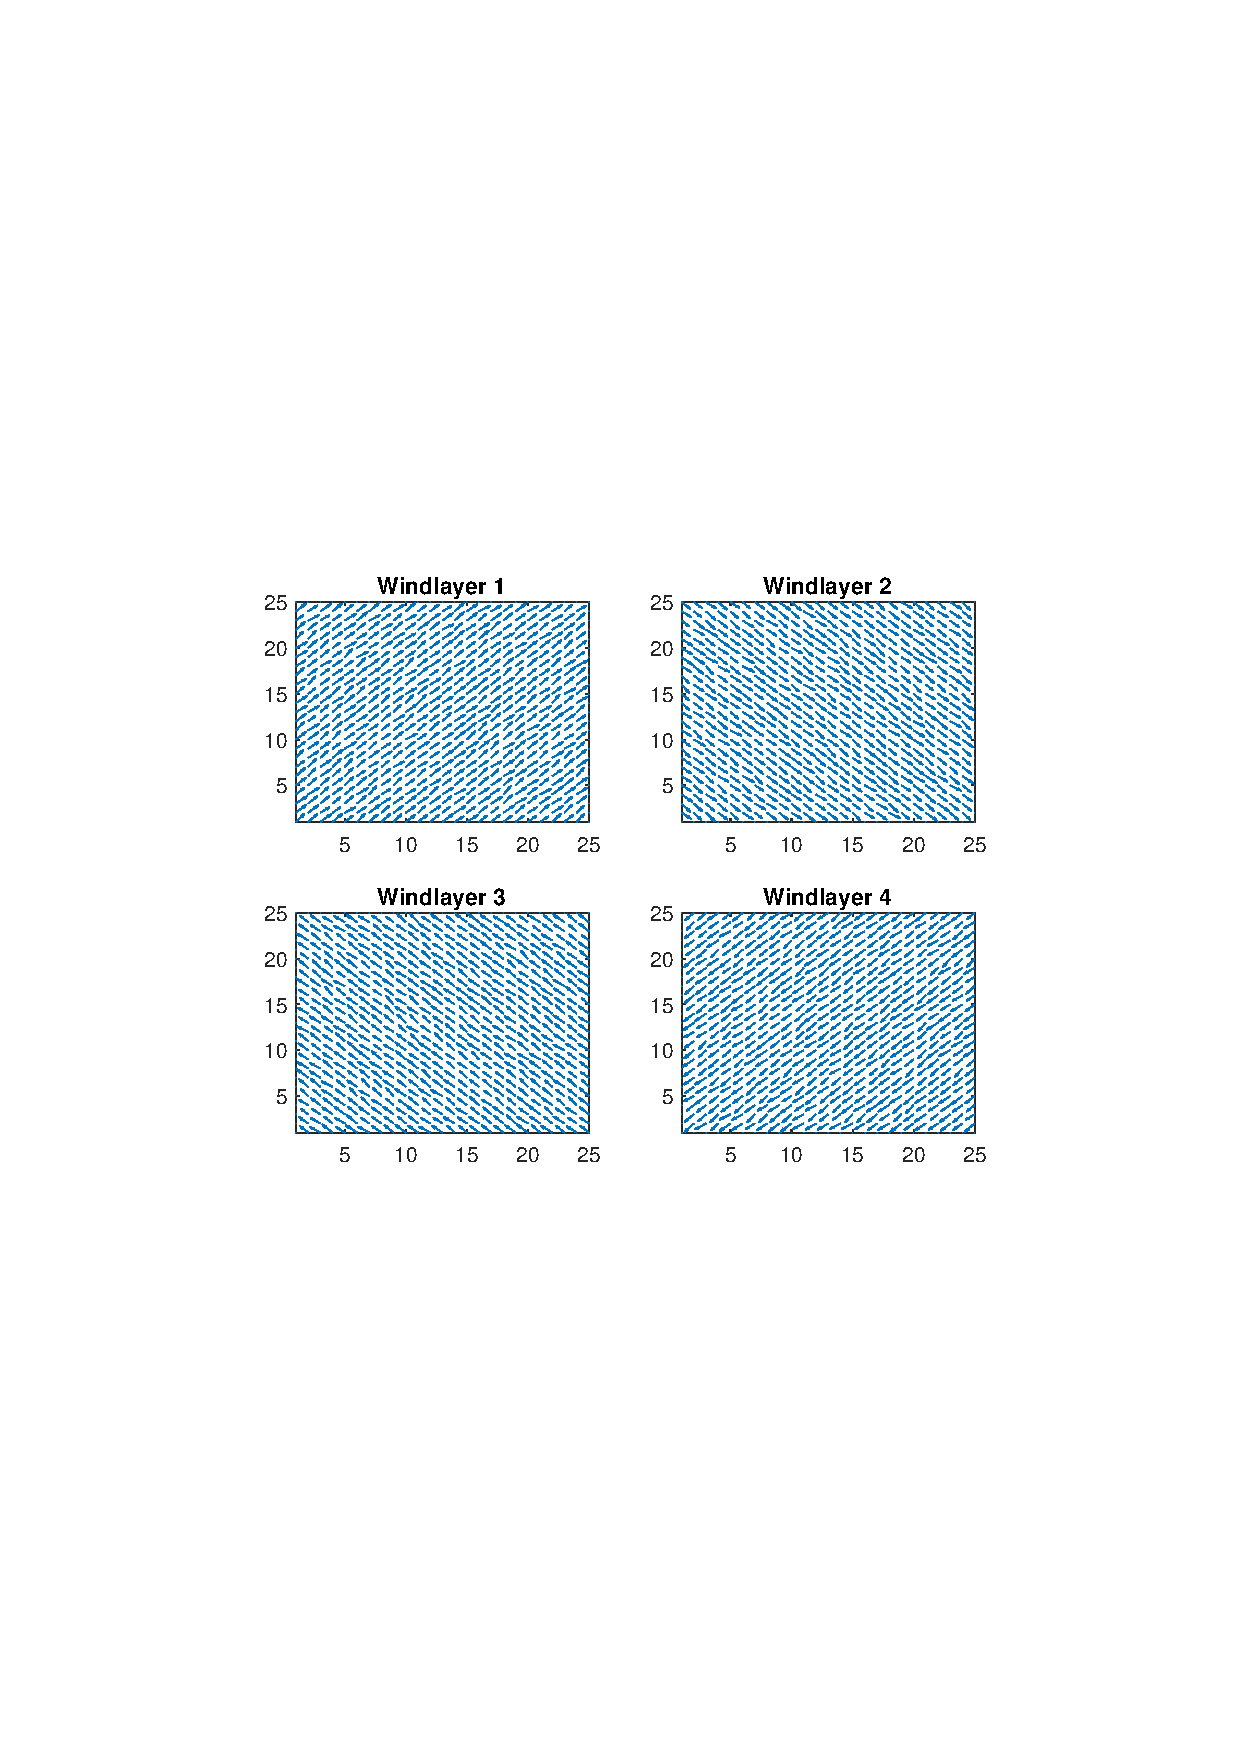
\includegraphics[width=\textwidth, trim={4cm 10cm 4cm 9cm},clip]{graphics/WindLayers.pdf}
\label{fig:windLayers}
\caption{Wind Layers}
\end{figure}


The stratosphere in the model is a collection of four layers, each with its own collection of wind vectors. The general direction of each is the same throughout the plane, but each vector has a deviation of about 10\% to make the behaviour realistic and give the control algorithms more directions to choose from. Each of the four layers have their own general direction, pointed towards one corner of the grid. This is done to increase variety of wind directions and possibilities to choose from. The average speed of the jet streams in the stratosphere is about miles an hour, or approximately 45 meters per second \citep{Roginsky1999}, which is used as a default size for the wind vectors. Figure \ref{fig:windLayers} shows an example of generated mock data set.

